\newcommand{\ptset}[1]{\ensuremath{\{\ldots,\vec{p}_{#1}\}}}
\newcommand{\codesnippet}[1]{\vspace{0.75em}\\
	$\left\langle\textit{#1}\right\rangle+\hspace{-4pt}\equiv$
	\vspace{-0.75em}
}
\newcommand{\codesnippetinl}[1]{
	$\left\langle\textit{#1}\right\rangle$
}
\chapter{Light Transport Modello e Surface Reflection}\label{chapter8}
Come gi\`a accennato in Capitolo \ref{chapter3}, ci\`o che rende difficile la risoluzione della Rendering Equation \`e il suo legame implicito con
la scena attraverso la ray tracing function $t(\vec{p}, \hat{\omega})$. L'irradianza spettrale risultante su un punto della superficie potrebbe 
presentare particolari tinte causate dall'illuminazione indiretta proveniente da un'altra superficie, e a sua volta entrambe sono illuminate da 
diverse sorgenti luminose. Gli algoritmi di rendering che considerano le mutue interazioni tra le superfici sono detti algoritmi di 
\textit{global illumination}, mentre algoritmi che fanno uso solo delle informazioni locali alla superficie analizzata algoritmi di 
\textit{local illumination}.\par
Gli algoritmi di Monte Carlo forniscono uno strumento potente per risolvere l'equazione di rendering, qui ripetuta
\begin{equation*}
	L_o(\vec{p},\hat{\omega}_o)=L_e(\vec{p},\hat{\omega}_o)+\int_{\mathcal{S}^s}f_s(\vec{p},\hat{\omega}_o,\hat{\omega}_i)L_i(\vec{p},\hat{\omega}_i)%
		\vert\langle\hat{n},\hat{\omega}_i\rangle\vert\mathrm{d}\hat{\omega}_i
\end{equation*}
La quale pu\`o essere risolta analiticamente solo nei casi pi\`u banali, ad esempio nel caso di una superficie lambertiana, dunque con BRDF pari a 
\mbox{$f_r(\vec{p},\hat{\omega}_o,\hat{\omega}_i)=\rho_{hh}/\pi$}, per la quale la radianza 
incidente ed emessa sono uguali in tutti i punti e direzioni della superficie. Utilizzando tale ipotesi e sostituendo 
\begin{equation*}
	L(\vec{p},\hat{\omega})=L_o(\vec{p},\hat{\omega})=L_i(\vec{p},-\hat{\omega})
\end{equation*}
Posso scrivere
\begin{equation}
	L=L_e+\rho_{hh}L=L_e+\rho_{hh}(L_e+\rho_{hh}(L_e+\ldots))=\sum_{i=0}^\infty L_e\rho_{hh}^i
\end{equation}
Dato che $\rho_{hh}<1$ per la conservazione dell'energia, la serie converge a 
\begin{equation}
	L=\frac{L_e}{1-\rho_{hh}}
\end{equation}
\begin{figure}[tb]
	\centering
	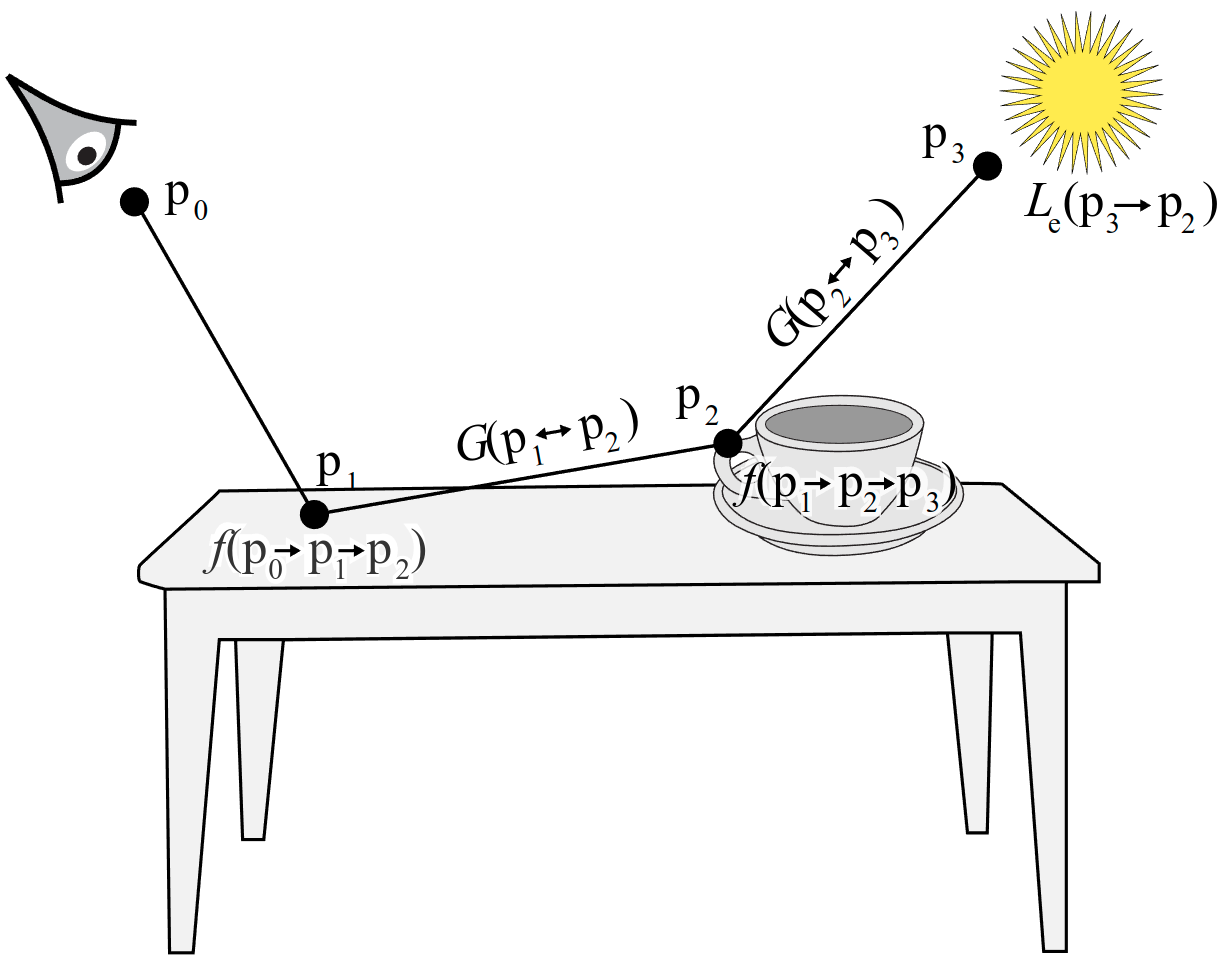
\includegraphics[width=0.8\linewidth]{../assets/chapter8_light_transport_equation.png}
	\caption{Illustrazione della Forma orientata su integrali di percorsi della rendering equation. Immagine da \cite{pharr}}
	\label{chapter8:LTE:pathFig}
\end{figure}
\section{Path Integral della Rendering Equation}
Abbiamo espresso, con Equazione \ref{chapter3:surface:areaRenderingEq}, la rendering equation in termini dell'unione di tutte le porzioni di 
superfici visibili dal punto $\vec{p}$, qui riportata
\begin{equation*}
	L(\vec{p},\hat{pq}) %
		= L_e(\vec{p},\hat{pq}) + \int_{A}f_s(\vec{p},\hat{\omega}_o,\hat{pq})G(\vec{p},\vec{q})L(\vec{q},-\hat{pq})\mathrm{d}A(\vec{q})
\end{equation*}
Si noti che un'equazione di questo tipo ha struttura nota come \textit{Equazione Integrale di Fredholm del secondo tipo}.\\
Definendo notazione \mbox{$L_{o|e}(\vec{p}_{i+1}\to\vec{p}_i)=L_{o|e}(\vec{p}_{i+1},\widehat{p_ip_{i+1}})$} e \\
\mbox{$f_r(\vec{p}_i,\vec{p}_{i+1},\vec{p}_{i+2})=f_r(\vec{p}_{i+1},\widehat{p_ip_{i+1}},\widehat{p_{i+1},p_{i+2}})$}, 
posso riscrivere tale equazione nella 
\textit{three-point form}
\begin{equation}\label{chapter8:LTE:3pointform}
	L(\vec{p}_1\to\vec{p}_0) %
		= L_e(\vec{p}_1\to\vec{p}_0)+\int_{A}f_s(\vec{p}_0,\vec{p}_1,\vec{p}_2)G(\vec{p}_1,\vec{p}_2)L(\vec{p}_2\to\vec{p}_1)\mathrm{d}A(\vec{p}_2)
\end{equation}
Dove ricordiamo il termine geometrico che lega le varie superfici \`e dato da Equazione \ref{chapter3:surface:geometricTerm}. La differenza tra 
la Rendering Equation sulla sfera di direzioni e questa forma consiste nel fatto che per valutare la prima, campioneremmo da una distribuzione di 
direzioni per generare raggi e valutare la funzione integranda ricorsivamente. In questa forma, campioneremmo punti sulle superfici seguendo una 
distribuzione sulle aree, ne calcoleremmo il termine geometrico, e genereremmo raggi per valutare la funzione di visibilit\`a 
\mbox{$V(\vec{p}_i,\vec{p}_{i+1})$}.\par 
La forma pi\`u flessibile della Equazione \ref{chapter8:LTE:3pointform} consiste in una formulazione che esprime la radianza come un integrale su 
dei percorsi, rappresentati come punti in uno spazio con alta dimensionalit\`a (vedi Figura \ref{chapter8:LTE:pathFig}), il quale ci permette di 
stabilire strategie sulla scelta di paths da valutare per poter sviluppare algoritmi efficienti. Per poter esplicitare tale forma espandiamo la 
definizione ricorsiva di radianza, e raggruppiamo i termini per complessit\`a
\begin{align}
	L(\vec{p}_1\to\vec{p}_0)&=L_e(\vec{p}_1\to\vec{p}_0) \nonumber \\
		&+\int_{A}L_e(\vec{p}_2\to\vec{p}_1)f_s(\vec{p}_0,\vec{p}_1,\vec{p}_2)G(\vec{p}_1,\vec{p}_2)\mathrm{d}A(\vec{p}_2) \nonumber \\
		&+\int_{A}\int_{A}L_e(\vec{p}_3\to\vec{p}_2)f_s(\vec{p}_1,\vec{p}_2,\vec{p}_3)G(\vec{p}_2,\vec{p}_3) \nonumber \\
		&\;\;\;\;\;\;\;\;\;\;\;\;\times f_s(\vec{p}_0,\vec{p}_1,\vec{p}_2)G(\vec{p}_1,\vec{p}_2)\mathrm{d}A(\vec{p}_2)\mathrm{d}A(\vec{p}_3) \nonumber\\
		&+\ldots \nonumber \\
		&=\sum_{i=1}^\infty P(\ptset{n})
\end{align}
Dove $\ptset{n}=\{\vec{p}_0,\vec{p}_1,\ldots,\vec{p}_n\}$.\par
$P(\ptset{n})$ restituisce la quantit\`a di radianza scattered lungo un percorso con 
gli $n+1$ vertici $\vec{p}_0,\vec{p}_1,\ldots,\vec{p}_n$, nei quali assumiamo $\vec{p}_0$ \`e sul film plane e $p_n$ \`e su una sorgente luminosa, 
pari a 
\begin{align}
	P(\ptset{n}) &= \nonumber\\&\underbrace{\int_A\int_A\ldots\int_A}_{n-1\text{ volte}}L_e(\vec{p}_n\to\vec{p}_{n-1})\left(\prod_{i=1}^{n-1}%
		f_s(\vec{p}_{i-1},\vec{p}_i,\vec{p}_{i+1})G(\vec{p_{i+1},p_{i}})\right)\mathrm{d}A(\vec{p}_2)\ldots\mathrm{d}A(\vec{p}_n) \\
	P(\ptset{0}) &= L_e(\vec{p}_1,\vec{p}_0) \nonumber
\end{align}
La produttoria evidenziata nell'n-esimo path integral \`e detta \textit{throughput} della path
\begin{equation}
	T(\ptset{n})=\prod_{i=1}^{n-1}f_s(\vec{p}_{i-1},\vec{p}_i,\vec{p}_{i+1})G(\vec{p_{i+1},p_{i}})
\end{equation}
Da cui 
\begin{equation}
	P(\ptset{n}) = \underbrace{\int_A\int_A\ldots\int_A}_{n-1\text{ volte}}L_e(\vec{p}_n\to\vec{p}_{n-1})T(\ptset{n})%
		\mathrm{d}A(\vec{p}_2)\ldots\mathrm{d}A(\vec{p}_n)
\end{equation}
Notiamo che dei termini $P(\ptset{i})$ potrebbero contenere distribuzioni di Dirac all'interno della loro funzione integranda, dovuta o a determinati 
modelli di sorgenti luminose o BSDF. Dunque le implementazioni devono gestire tale caso particolare in quanto riduce la quantit\`a di termini della 
somma da stimare. Si consideri l'esempio da \cite{pharr} per l'illuminazione diretta con una sorgente puntiforme descritta da una distribuzione di 
Dirac.\par
Un approccio per partizionare la somma infinita di path integrals \`e la seguente:
\begin{equation}
	L(\vec{p}_1\to\vec{p}_0)=P(\ptset{1})+P(\ptset{2})+\sum_{i=3}^\infty P(\ptset{i})
\end{equation}
Dove il primo termine \`e calcolato facilmente valutando la radianza emessa dal punto $\vec{p}_1$ verso $\vec{p}_0$, il secondo integrale \`e stimato 
con accuratezza elevata e i restanti termini della somma sono stimati con un'approssimazione pi\`u grossolana. Inoltre, si potrebbero anche partizionare
gli integrali a seconda della categoria di sorgenti luminose e BSDF, ad esempio per distinguere sorgenti grandi da sorgenti piccole, e BSDF contenenti
$\delta(x)$ dal resto.
\section{Path Tracing}
Avendo ricavato una espressione facilmente manovrabile, siamo pronti a formulare un'algoritmo per la risoluzione dell'equazione di Rendering.\par
Chiaramente nella nostra computazione non abbiamo la possibilit\`a di valutare una serie, per cui applichiamo \textit{Russian Roulette} 
(\ref{chapter6:variance:russianRoulette}), valutando la terminazione della valutazione della serie ad ogni termine com probabilit\`a $q_i$, definite 
a priori. Un approccio per la scelta di tali probabilit\`a \`e la seguente (giustificata in \cite{pharr})
\begin{align}
	q_j&\sim\mathcal{U}\left(0,1-\max_{\lambda\in\Lambda}\left\{
		\eta\prod_{i=1}^{j-2}\frac{f_s(\vec{p}_{j-1},\vec{p}_j,\vec{p}_{j+1})}{p_\omega(\hat{\omega}_j)}\right\}\right)
\end{align}
dove $\hat{\omega}_j=(\vec{p}_{j+1}-\vec{p}_j)/\norm{\vec{p}_{j+1}-\vec{p}_j}$ e $p_\omega(\hat{\omega}_j)$ PDF della BSDF 
(\ref{chapter3:surface:brdf})\par
Applicando la compensazione per tale tecnica, lo stimatore unbiased diventa
\begin{equation}\label{chapter8:pt:russianroulette}
	\frac{1}{1-q_1}\left(P(\ptset{1})+\frac{1}{1-q_2}\left(P(\ptset{2})+\frac{1}{1-q_3}\left(P(\ptset{3})+\ldots\right)\right)\right)
\end{equation}
In quanto il throughput totale della path
\begin{equation*}
	\beta=\prod_{i=1}^{j-2}\frac{f_s(\vec{p}_{j-1},\vec{p}_j,\vec{p}_{j+1})}{p_\omega(\hat{\omega}_j)}
\end{equation*}
decresce man mano che il tracing continua, \`e garantito che la valutazione della path termini in un tempo limitato. Si noti che nonostante Russian
Roulette aumenta l'MSE, in quanto si accumulano meno contributi, l'efficienza aumenta comunque per la notevole diminuzione del Running Time.\par
Per stimare ciascun path integral $P(\ptset{n})$, necessitiamo di $n+1$ vertici dei quali $\vec{p}_0$ sia sul film plane e $\vec{p}_n$ sia su una 
sorgente luminosa. Un approccio potrebbe essere campionare, dopo aver scelto il vertice sul film plane da cui partire, $n-2$ punti da tutte le 
superfici della scena con densit\`a di distribuzione uniforme, e l'ultimo campione su una delle superfici luminose presenti nella scena con equa
probabilit\`a. Tale approccio per\`o non conta la mutua visibilit\`a tra le superfici e pu\`o condurre a risultati con alta varianza, per via della 
presenza di paths con contributo nullo, e risultati incorretti, senza contare il fatto che tale metodo non supporta una gestione per le distribuzioni
contenenti il delta di Dirac. Una strategia valida \`e rappresentata invece dalla \textit{Costruzione Incrementale del percorso} \cite{pharr}:\par
partendo da un punto del film plane $\vec{p}_0$ (per il quale la direzione del raggio visivo \`e determinata geometricamente dal camera model),
si traccia un raggio per intersecare una superficie in $\vec{p}_1$. Da qui si ripete il procedimento descritto a seguire.\par
da $\vec{p}_i$ campiona una direzione dalla BSDF per ottenere una direzione $\hat{\omega}_i$ la quale, tracciato un raggio lungo essa, che conduce ad 
una nuova intersezione $\vec{p}_{i+1}$.\par
L'ultimo punto del path $\vec{p}_n$ deve terminare su una sorgente luminosa. L'approccio utilizzato per la determinazione della sorgente da utilizzare
\`e il Multiple Importance Sampling, utilizzando come densit\`a di distribuzione la PDF della BSDF dell'ultima superficie, $p_\omega$, e la PDF 
della sorgente luminosa selezionata per il calcolo della radianza uscente dall'ultima superficie, $p_l$. Si ricordi che tali PDF hanno come dominio
la sfera unitaria di possibili direzioni, ed 
in quanto il path integral \`e un integrale su un area, bisogna applicare la correzione (vedi Equazione \ref{chapter3:surface:areaRenderingEq})
\begin{equation}
	p_A(\vec{p}_i)=p_\omega(\hat{\omega}_{j-1})\frac{|\langle\hat{n},\hat{p}_i\rangle|}{\norm{\vec{p}_{i-1}-\vec{p}_i}^2}
\end{equation}
andandosi a semplificare con il termine geometrico\footnote{omesso l'Importance Sampling per semplicit\`a e per evidenziare i passaggi seguiti}
\begin{align}
	P(\ptset{n})&\approx L_e(\vec{p}_n\to\vec{p}_{n-1})\prod_{i=1}^{n-1}\frac{f_s(\vec{p}_{i-1},\vec{p}_i,\vec{p}_{i+1})G(\vec{p_{i+1},p_{i}})}
		{p_A(\vec{p}_{i+1})} \nonumber \\
	&=L_e(\vec{p}_n\to\vec{p}_{n-1})\prod_{i=1}^{n-1}\frac{f_s(\vec{p}_{i-1},\vec{p}_i,\vec{p}_{i+1})V(\vec{p}_{i+1},\vec{p}_i)
		\frac{|\cos\theta_{i+1}||\cos\theta_i|}{\norm{\vec{p}_{i+1}-\vec{p}_i}^2}}{p_A(\vec{p}_{i+1})} \nonumber \\
	&=L_e(\vec{p}_n\to\vec{p}_{n-1})\prod_{i=1}^{n-1}\frac{f_s(\vec{p}_{i-1},\vec{p}_i,\vec{p}_{i+1})V(\vec{p}_{i+1},\vec{p}_i)
		\frac{|\cos\theta_{i+1}||\cos\theta_i|}{\norm{\vec{p}_i-\vec{p}_{i+1}}^2}}
		{p_\omega(\omega_i)\frac{|\cos\theta_{i+1}|}{\norm{\vec{p}_i-\vec{p}_{i+1}}^2}} \nonumber \\
	&=L_e(\vec{p}_n\to\vec{p}_{n-1})\prod_{i=1}^{n-1}\frac{f_s(\vec{p}_{i-1},\vec{p}_i,\vec{p}_{i+1})V(\vec{p}_{i+1},\vec{p}_i)
		|\cos\theta_i|}{p_\omega(\omega_i)}
\end{align}
Dopodich\`e suddividiamo il termine di Direct Lighting applicando MIS
\begin{align}
	P(\ptset{i})&\approx w_l(\hat{\omega}_l)\frac{L_e(\vec{p}_l\to\vec{p}_{i-1})f_s(\vec{p}_{i-2},\vec{p}_{i-1},\vec{p}_l)
		|\cos\theta_l|V(\vec{p}_{i-1},\vec{p}_l)}{p_l(\hat{\omega}_l)}\beta \nonumber \\
	&+w_b(\hat{\omega}_e)\frac{L_e(\vec{p}_b\to\vec{p}_{i-1})f_s(\vec{p}_{i-2},\vec{p}_{i-1},\vec{p}_b)
		|\cos\theta_b|V(\vec{p}_{i-1},\vec{p}_b)}{p_b(\hat{\omega}_b)}\beta
\end{align}
dove i pesi sono calcolati con la \textit{balance heuristic} o la \textit{power heuristic} (Sezione \ref{chapter6:variance:importanceSampling}).\par
L'algoritmo completo implementante le tecniche qui discusse pu\`o essere trovato in \cite{pharr}.
\section{Applicazione del Metodo di Monte Carlo: Esempio Path Tracing Semplificato}
Al fine di chiarificare come tali metodologie sono applicate in pratica, si propone di seguito un Path Tracer semplificato, supportante
\begin{figure}[tb]
	\centering
	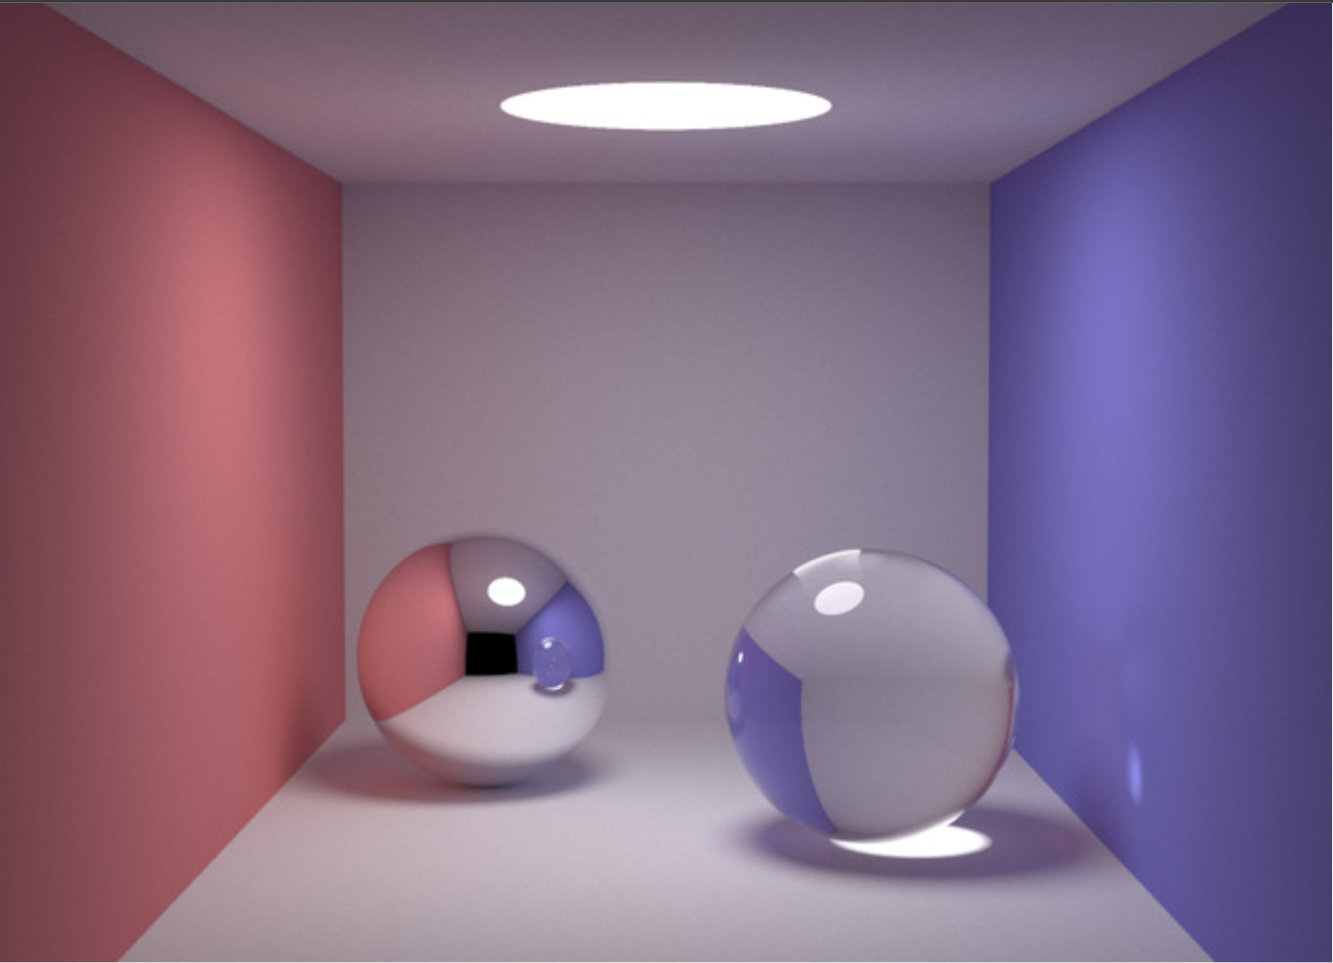
\includegraphics[width=0.7\linewidth]{../assets/chapter8_MCRendering_reference.png}
	\caption{Cornell Box scene utilizzata per il test.}
	\label{chapter8:MCRendering:reference}
\end{figure}
\begin{itemize}[topsep=0pt,noitemsep]
	\item Tre tipi di BRDF, in particolare Lambertiana (\textrm{DIFF}), Speculare opaca (\textrm{SPEC}), Speculare traslucente (\textrm{REFL}) 
	\item Russian Roulette, applicata per terminare la valutazione di una path e per scegliere tra riflessione o trasmissione nel caso di 
		BRDF traslucente
	\item Stratified Sampling, dividendo ciascun pixel cell in 4 caselle, e campionando per ciascuna di esse un numero di samples pari all'input da 
		linea di comando. 
	\item Ciascun sample in ciascun strata \`e scelto casualmente con PDF triangolare
\end{itemize}
Il quale crea una resa della celebre \textit{Cornell Box}, scena utilizzata per testare 3D rendering software creata e presentata nel SIGGRAPH 1984
(vedi Figura \ref{chapter8:MCRendering:reference}).\par
In questa implementazione, la scena \`e composta esclusivamente da sfere, definite attraverso un raggio, posizione, radianza emessa, 
riflettanza spettrale (formalmente DHR o albedo, Equazione \ref{chapter3:surface:DHR}, informalmente "colore"), tipologia di materiale.
\codesnippet{Definizione \textrm{Sphere} struct}
\begin{minted}[tabsize=2,obeytabs,escapeinside=¬¬,mathescape=true]{C++}
	struct Sphere { 
	  double rad;
	  Vec p, e, c;
	  Refl_t refl;      
	 ¬\codesnippetinl{Costruttore (\ref{appendixD:pathTracer})}¬
	 ¬\codesnippetinl{Metodo per intersezione (\ref{appendixD:pathTracer})}¬
	}; 
\end{minted}
Da cui possiamo definire i lati del cubo come sfere con raggio elevato, la sorgente luminosa come sfera con radianza emessa non nulla riflettanza 
spettrale nulla, e le comuni sfere, con radianza emessa nulla e riflettanza spettrale non nulla, definente la tinta del materiale
\codesnippet{Definizione della scena}
\begin{minted}[tabsize=2,obeytabs,escapeinside=¬¬,mathescape=true]{C++}
	Sphere spheres[] = {
	  Sphere(1e5, Vec( 1e5+1,40.8,81.6), Vec(),Vec(.75,.25,.25),DIFF),
	  Sphere(1e5, Vec(-1e5+99,40.8,81.6),Vec(),Vec(.25,.25,.75),DIFF),
	  Sphere(1e5, Vec(50,40.8, 1e5),     Vec(),Vec(.75,.75,.75),DIFF),
	  Sphere(1e5, Vec(50,40.8,-1e5+170), Vec(),Vec(),           DIFF),
	  Sphere(1e5, Vec(50, 1e5, 81.6),    Vec(),Vec(.75,.75,.75),DIFF),
	  Sphere(1e5, Vec(50,-1e5+81.6,81.6),Vec(),Vec(.75,.75,.75),DIFF),
	  Sphere(16.5,Vec(27,16.5,47),       Vec(),Vec(1,1,1)*.999, SPEC),
	  Sphere(16.5,Vec(73,16.5,78),       Vec(),Vec(1,1,1)*.999, REFR),
	  Sphere(600, Vec(50,681.6-.27,81.6),Vec(12,12,12),  Vec(), DIFF) 
	}; 
\end{minted}
Il codice parte nella funzione \texttt{main}, la quale opera nel seguente modo
\codesnippet{\texttt{main} outline}
\begin{minted}[tabsize=2,obeytabs,escapeinside=¬¬,mathescape=true]{C++}
	int main(int argc, char *argv[]) {
		// definisci risoluzione griglia film plane (schermo) e numero di campioni
		// per pixel da linea di comando
		int w=1024, h=768, samps = argc==2 ? atoi(argv[1])/4 : 1;

		// definisci posizione e direzione osservatore, utilizzando il
		// Pinhole Camera Model
		Ray cam(Vec(50,52,295.6), Vec(0,-0.042612,-1).norm());

		// definisci direzione orizzontale $\mathtt{cx}\text{ e verticale }\mathtt{cy}$
		// della camera. "%" e' definito come prodotto vettoriale $\mathrm{vedi}\;\ref{appendixD:pathTracer}$
		Vec cx=Vec(w*.5135/h), cy=(cx%cam.d).norm()*.5135;

		// variabile che conterra' la stima effettuata per ogni sample
		Vec r;

		// Buffer che conterra' l'immagine finale
		Vec* c=new Vec[w*h];

		// direttiva per la programmazione multicore con OpenMP
	#pragma omp parallel for schedule(dynamic, 1) private(r)
		// per ogni pixel
		for (int y=0; y<h; y++) {
			printf(stderr,"\rRendering (%d spp) %5.2f%%",samps*4,100.*y/(h-1));
			for (unsigned short x=0, Xi[3]={0,0,y*y*y}; x<w; x++)
			  ¬\codesnippetinl{Calcola il colore mostrato dal pixel}¬
		} 

		// salva l'immagine sintetizzata in un file
		FILE *f = fopen("image.ppm", "w");
		fprintf(f, "P3\n%d %d\n%d\n", w, h, 255);
		for (int i=0; i<w*h; i++)
			fprintf(f,"%d %d %d ", toInt(c[i].x), toInt(c[i].y), toInt(c[i].z));
	} 
\end{minted}
\begin{figure}[tb]
	\centering
	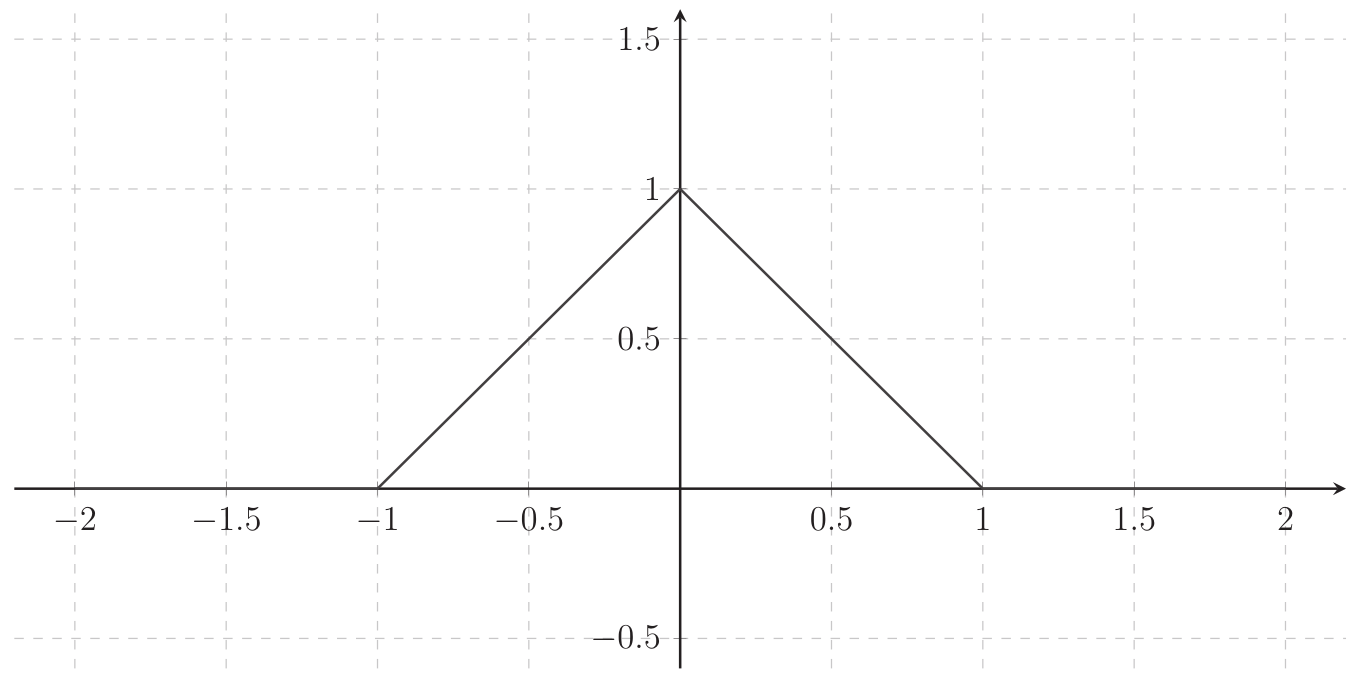
\includegraphics[width=0.6\linewidth]{../assets/chapter8_triangular_function.png}
	\caption{Grafico funzione triangolare $\wedge(x)$. Immagine da \cite{pegoraro}}
\end{figure}
Per ogni pixel cell, ciascuno dei quattro strata viene campionato con un numero di samples pari all'input dato al programma in console (default: $1$),
con PDF pari alla funzione triangolare normalizzata, cio\`e
\begin{align}
	f(x,y)&=\wedge(x)\wedge(y) \\
	\wedge(x)&=\max\{0,1-|x|\}\nonumber
\end{align}
Da cui Inverse Transform Sampling pu\`o essere applicato calcolandone CDF separabile
\begin{equation}
	2\int_0^{t_s}\wedge(t)\mathrm{d}t=2\int_0^{t_s}1-|t|\mathrm{d}t=2\left[t-\frac{t^2}{2}\right]_{t=0}^{t_s}=t_s(2-t_s)
\end{equation}
e invertendola, dato un $\xi\sim\mathcal{U}(0,1)$ (vedi Sezione \ref{chapter6:sampling:inverseTransformSection})
\begin{equation}
	\xi=t_s(2-t_s)\longrightarrow t_s=1-\sqrt{1-\xi}
\end{equation}
Tale espressione pu\`o essere utilizzata per calcolare ascissa e ordinata del subpixel sample
\codesnippet{Calcola il colore mostrato dal pixel}
\begin{minted}[tabsize=2,obeytabs,escapeinside=¬¬,mathescape=true]{C++}
	// per ogni strata
	for (int sy=0, i=(h-y-1)*w+x; sy<2; sy++)     
		for (int sx=0; sx<2; sx++, r=Vec()){        
			// per ogni campione nello strata
			for (int s=0; s<samps; s++){ 
				// genera un numero casuale basato sul seed $\mathtt{Xi}$ con PDF 
				// triangolare per ogni coordinata del campione...
				double r1=erand48(Xi), dx=1-sqrt(1-r1); 
				double r2=erand48(Xi), dy=1-sqrt(1-r2); 

				// ...e utilizzalo come scostamento dal centro dello strata 
				// (tecnica nota come $\textit{jittering}$), tramite il quale possiamo
				// definire la direzione del raggio da proiettare dall'osservatore, di 
				// posizione $\mathtt{cam.o}$
				Vec d = cx*( ( (sx+.5 + dx)/2 + x)/w - .5) 
					  + cy*( ( (sy+.5 + dy)/2 + y)/h - .5) + cam.d; 

				¬\codesnippetinl{Applica lo Stimatore di Monte Carlo}¬
			} 

			// Il colore finale del pixel e' pari alla media dei quattro colori 
			// calcolati per ogni strata
			c[i] = c[i] + Vec(clamp(r.x),clamp(r.y),clamp(r.z))*.25; 
		} 
\end{minted}
Dove giungiamo finalmente all'applicazione dell'Equazione \ref{chapter6:MC:crudeEstimator}
\codesnippet{Applica lo Stimatore di Monte Carlo}
\begin{minted}[tabsize=2,obeytabs,escapeinside=¬¬,mathescape=true]{C++}
	r = r + radiance(Ray(cam.o+d*140,d.norm()),0,Xi)*(1./samps); 
\end{minted}
Dove la funzione \texttt{radiance} \`e una funzione ricorsiva, che ritorna un campione della funzione immagine, i cui parametri sono
\begin{itemize}[topsep=0pt,noitemsep]
	\item Raggio da proiettare
	\item \textit{ray depth} corrente, ovvero il numero di "rimbalzi" gi\`a effettuati
	\item seed per RNG
	\item booleano che indica se contare radianza emessa o meno (default: \texttt{true})
\end{itemize}
La cui definizione \`e la seguente
\codesnippet{Funzione $\mathtt{radiance}$}
\begin{minted}[tabsize=2,obeytabs,escapeinside=¬¬,mathescape=true]{C++}
	Vec radiance(const Ray &r, int depth, unsigned short *Xi){ 
		double t;
		int id=0;
		if (!intersect(r, t, id)) return Vec();

		const Sphere &obj = spheres[id]; 

		/*
		 * Rispettivamente:
		 * x  <- punto di intersezione tra sfera e raggio
		 * n  <- normale della sfera
		 * nl <- normale riorientata per formare un angolo acuto con l'osservatore
		 * f  <- riflettanza della sfera, modula il contributo della BRDF
		 */
		Vec x=r.o+r.d*t, n=(x-obj.p).norm(), nl=n.dot(r.d)<0?n:n*-1, f=obj.c;

		// Applica Russian Roulette per tutti i raggi con depth > 5, dunque 
		// - Dalla quinta superficie intersecata in poi, con probabilita' $\mathtt{p}$.
		// - Applica la compensazione (Equazione $\ref{chapter8:pt:russianroulette}$) in caso il raggio persista.
		// - Confronta la probabilita' estratta con la componente massima della 
		//   riflettanza per decidere se terminare il raggio o meno
		double p = f.x>f.y && f.x>f.z ? f.x:
		                      f.y>f.z ? f.y:
		                                f.z;
		if (++depth>5) {
			if (erand48(Xi)<p) f=f*(1/p); 
			else return obj.e;
		}

		// Se la sfera ha BRDF lambertiana
		if (obj.refl == DIFF) {
			¬\codesnippetinl{Calcola contributo per BRDF Lambertiana e reitera}¬
		} 

		// Se la sfera ha BRDF speculare opaca
		else if (obj.refl == SPEC)
			¬\codesnippetinl{Calcola contributo per BRDF Speculare Opaca e reitera}¬

		// Se la sfera ha BRDF speculare translucente
  ¬\codesnippetinl{Calcola contributo per BRDF Speculare Translucente e reitera}¬
	}
\end{minted}
In tutti e tre i casi di BRDF, il risultato \`e pari alla radianza emessa sommata alla radianza riflessa/trasmessa, come prescrive 
la Rendering Equation (Equazione \ref{chapter3:surface:renderingEq}). Per quest'ultima, si esegue una chiamata ricorsiva alla funzione 
\texttt{radiance}, con direzione campionata dipendente dalla BRDF in questione.\par
Per una BRDF lambertiana, Equazione \ref{chapter3:surface:lambert}, il campionamento pu\`o seguire una cosine-lobe distribution di grado $1$, 
approccio illustrato in Equazione \ref{chapter3:surface:cosineLobeSampling}.\par
In quanto un approccio basato sui path presentato nelle sezioni precedenti richiederebbe un codice molto lungo, ci limitiamo a seguire un approccio
basato sulle direzioni, e supponendo BRDF Lambertiana la Rendering Equation diventa
\begin{align}
	L_o(\vec{p},\hat{\omega}_o)&=L_e(\vec{p},\hat{\omega}_o)+\int_{\mathcal{H}^2(\hat{n})}%
		L_i(\vec{p},\hat{\omega}_i)\frac{\rho(\vec{p})}{\pi}\langle\hat{n},\hat{\omega}_i\rangle\mathrm{d}\hat{\omega}_i\nonumber\\
	&=L_e(\vec{p},\hat{\omega}_i)+\frac{\rho(\vec{p})}{\pi}\int_{\mathcal{H}^2(\hat{n})}%
		L_i(\vec{p},\hat{\omega}_i)|\langle\hat{n},\hat{\omega}_i\rangle|\mathrm{d}\hat{\omega}_i\nonumber\\
\end{align}
applicando lo stimatore di Monte Carlo con un singolo campione ($n=1$)
\begin{align}
	L_o(\vec{p},\hat{\omega}_o)&\approx L_e(\vec{p},\hat{\omega}_o)+\frac{\norm{\mathcal{H}^2(\hat{n})}}{n}\frac{\rho}{\pi}
		\frac{L_i(\vec{p},\hat{\omega})|\langle\hat{n},\hat{\omega}\rangle|}{p_\omega(\hat{\omega})}\nonumber \\
	&=L_e(\vec{p},\hat{\omega}_o)+\rho\frac{L_i(\vec{p},\hat{\omega})|\langle\hat{n},\hat{\omega}\rangle|}{p_\omega(\hat{\omega})}
\end{align}
Che \`e l'equazione implementata nella riga finale del seguente codice
\codesnippet{Calcola contributo per BRDF Lambertiana e reitera}
\begin{minted}[tabsize=2,obeytabs,escapeinside=¬¬,mathescape=true]{C++}
	// $\phi$, angolo azimuthale (Figura $\ref{chapter3:surface:projectedArea}$)
	double r1=2*M_PI*erand48(Xi);

	// $\sin\theta$, dove $\theta$ angolo rispetto allo zenith (Figura $\ref{chapter3:surface:projectedArea}$)
	double r2=erand48(Xi), r2s=sqrt(r2);

	/*
	 * definizione del sistema di riferimento con i tre versori
	 * w <- normale, direzione dello zenith
	 * u <- direzione tangente alla superficie
	 * v <- direzione bitangente alla superficie
	 */
	Vec w=nl, u=((fabs(w.x)>.1?Vec(0,1):Vec(1))%w).norm(), v=w%u;

	// conversione da coordinate sferiche a coordinate cartesiane
	Vec d = (u*cos(r1)*r2s + v*sin(r1)*r2s + w*sqrt(1-r2)).norm();

	// calcolo della radianza finale con ricorsione
	// ($\mathtt{f.mult}$ indica prodotto di Hadamard)
	return obj.e + f.mult(radiance(Ray(x,d),depth,Xi));
\end{minted}
Una BRDF speculare opaca non calcola alcuna direzione casuale, per via della distribuzione di Dirac presente nella sua BRDF 
(Equazione \ref{chapter3:BRDF:specular}), dunque riflette solamente nella direzione indicata in Equazione \ref{chapter3:surface:reflectedDirection}
\begin{align}
	L_o(\vec{p},\hat{\omega}_o)&=L_e(\vec{p},\hat{\omega}_o)+\int_{\mathcal{H}^2(\hat{n})}%
		L_i(\vec{p},\hat{\omega}_i)F_r(\vert\langle\hat{n},\hat{\omega}_o\rangle\vert)%
		\frac{\delta(\hat{\omega}_i-\hat{\omega}_r)}{\vert\langle\hat{n},\hat{\omega}_i\rangle\vert}
		\vert\langle\hat{n},\hat{\omega}_i\rangle\vert\mathrm{d}\hat{\omega}_i\nonumber\\
	&=L_e(\vec{p},\hat{\omega}_o)+F_r(\vert\langle\hat{n},\hat{\omega}_o\rangle\vert)L_i(\vec{p},\hat{\omega}_r)\nonumber\\
	&=L_e(\vec{p},\hat{\omega}_o)+\bar{F}_rL_i(\vec{p},\hat{\omega}_r)
\end{align}
Dove $\xoverline{F}_r$ indica il valor medio della Fresnel Reflectance, rappresentato dal parametro \texttt{c} memorizzato dalle \texttt{Sphere}s.
\codesnippet{Calcola contributo per BRDF Speculare Opaca e reitera}
\begin{minted}[tabsize=2,obeytabs,escapeinside=¬¬,mathescape=true]{C++}
	return obj.e + f.mult(radiance(Ray(x,r.d-n*2*n.dot(r.d)),depth,Xi));
\end{minted}
Infine, la BRDF speculare traslucente \`e pensata per modellare una superficie vetrosa. Infatti, il suo IOR \`e assunto pari a $\eta_t=1.5$, mentre 
si assume indice di rifrazione unitario per l'ambiente circostante. Le equazioni sono simili alle precedenti con l'aggiunta del termine di 
radianza trasmessa. Il funzionamento \`e il seguente:
\begin{enumerate}[topsep=0pt,noitemsep]
	\item calcola l'indice di rifrazione relativo, pari al rapporto IOR entrante e IOR uscente. Calcola anzi tempo la direzione riflessa
	\item Se si \`e nel caso di riflessione interna, si fa ricorsione con la direzione riflessa
	\item Altrimenti calcola anzi tempo la direzione trasmessa (Equazione \ref{chapter3:surface:refractedDirection})
	\item Calcola la riflettanza per la direzione di incidenza con l'approssimazione di Schlick, utilizzabile in quanto si sta supponendo vetro 
		come materiale, che \`e un dielettrico (Equazione \ref{chapter3:surface:schFresnel}).
	\item Calcola il contributo di raggio riflesso e raggio trasmesso
	\item Russian Roulette: se \texttt{depth} $> 2$, allora uno dei due raggi, riflesso o trasmesso, \`e terminato
\end{enumerate}
Il codice \`e il seguente:
\codesnippet{Calcola contributo per BRDF Speculare Translucente e reitera}
\begin{minted}[tabsize=2,obeytabs,escapeinside=¬¬,mathescape=true]{C++}
	// Calcola direzione riflessa
	Ray reflRay(x, r.d-n*2*n.dot(r.d));

	// calcola indice di rifrazione relativo e $\mathtt{ddn}=\langle\hat{n},\hat{\omega}_o\rangle$
	bool into = n.dot(nl)>0;
	double nc=1, nt=1.5, nnt=into?nc/nt:nt/nc, ddn=r.d.dot(nl)

	// test per riflessione interna totale
	double cos2t = 1-nnt*nnt*(1-ddn*ddn);
	if (cos2t<0)
		return obj.e + f.mult(radiance(reflRay,depth,Xi));

	// calcola direzione di trasmissione
	Vec tdir = (r.d*nnt - n*((into?1:-1)*(ddn*nnt+sqrt(cos2t)))).norm();

	// calcola coefficienti di fresnel di riflessione e trasmissione
	double a=nt-nc, b=nt+nc, R0=a*a/(b*b), c = 1-(into?-ddn:tdir.dot(n));
	double Re=R0+(1-R0)*c*c*c*c*c;
	double Tr=1-Re;

	// Applicazione Russian Roulette: se $\mathtt{depth}$ del raggio e' maggiore 
	// di 2, allora uno dei due raggi e' terminato. La scelta tra il raggio 
	// riflesso $\mathtt{reflRay}$ e raggio trasmesso $\mathtt{Ray(x,tdir)}$ e' 
	// dettata dalla riflettanza di Fresnel $\mathtt{Re}$: piu' e' alta, e piu' 
	// la probabilita' $\mathtt{P}$ di scegliere di terminare 
	// il raggio rifratto e' alta
	double P=.25+.5*Re;

	// Applica la compensazione prevista dalla tecnica Russian Roulette
	double RP=Re/P;
	double TP=Tr/(1-P);

	// Calcola il contributo di radianza finale
	return obj.e + f.mult(depth>2 ? (erand48(Xi)<P ? radiance(reflRay,depth,Xi)*RP:
	                                                 radiance(Ray(x,tdir),depth,Xi)*TP)
	                              : radiance(reflRay,depth,Xi)*Re 
	                                + radiance(Ray(x,tdir),depth,Xi)*Tr);
\end{minted}
I risultati dell'algoritmo sono mostrati in Figura \ref{chapter8:LT:results}, seguite da Tabella \ref{chapter8:LT:variances}. Quest'ultima riporta, 
per ogni simulazione eseguita, con numero differente di pixel per stratum, campionati con PDF triangolare, la varianza di ciascuna immagine risultante
per red channel, green channel, blue channel, e luminance channel. Quest'ultimo, in particolare, \`e stato calcolato per ogni pixel come luma channel 
definito dal color space standardizzato ITU BT.709 $YC_BC_R$
\begin{equation*}
	Y = 0.2126R+0.7152G+0.0722B
\end{equation*}
Si pone l'accento su esso in quanto sono visibili incrementi notevoli di qualit\`a dell'immagine ogni qual volta la varianza per 
tale canale diminuisce di $0.01$
\begin{figure}[p]
    \begin{subfigure}[c]{0.4\linewidth}
	\centering
	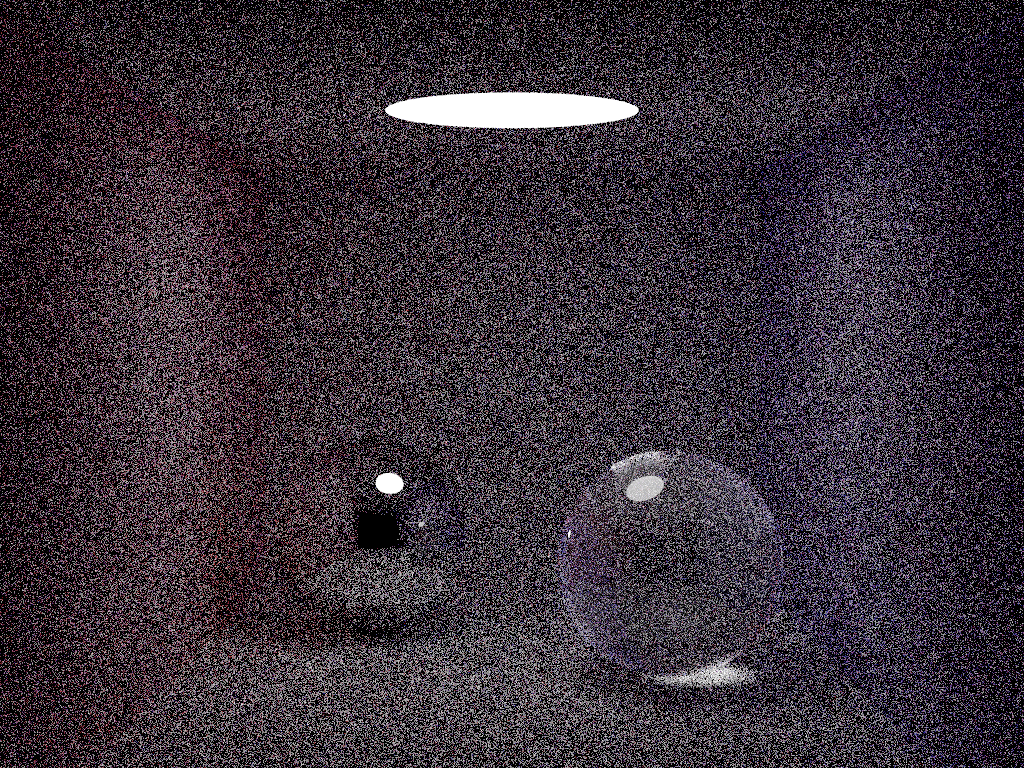
\includegraphics[width=\linewidth]{../assets/appendixD_result_8.png}
	\caption{8 campioni per stratum}
    \end{subfigure}\hspace{12pt}
    \begin{subfigure}[c]{0.4\linewidth}
	\centering
	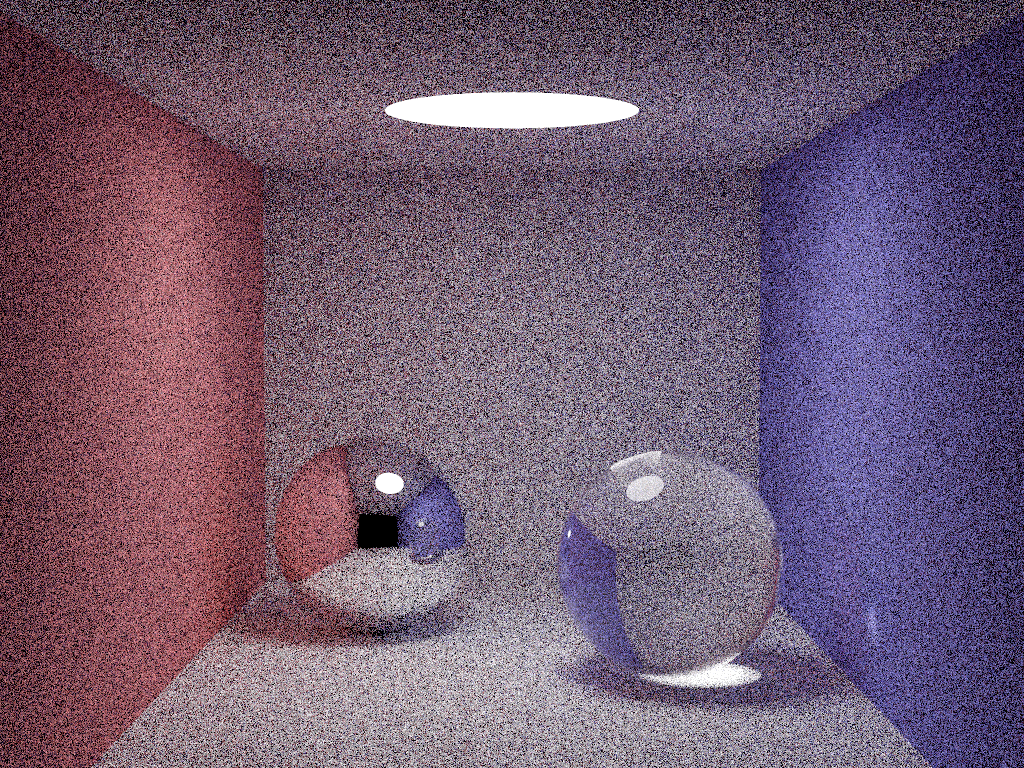
\includegraphics[width=\linewidth]{../assets/appendixD_result_40.png}
	\caption{40 campioni per stratum}
    \end{subfigure}\hfill
    \begin{subfigure}[c]{0.4\linewidth}
	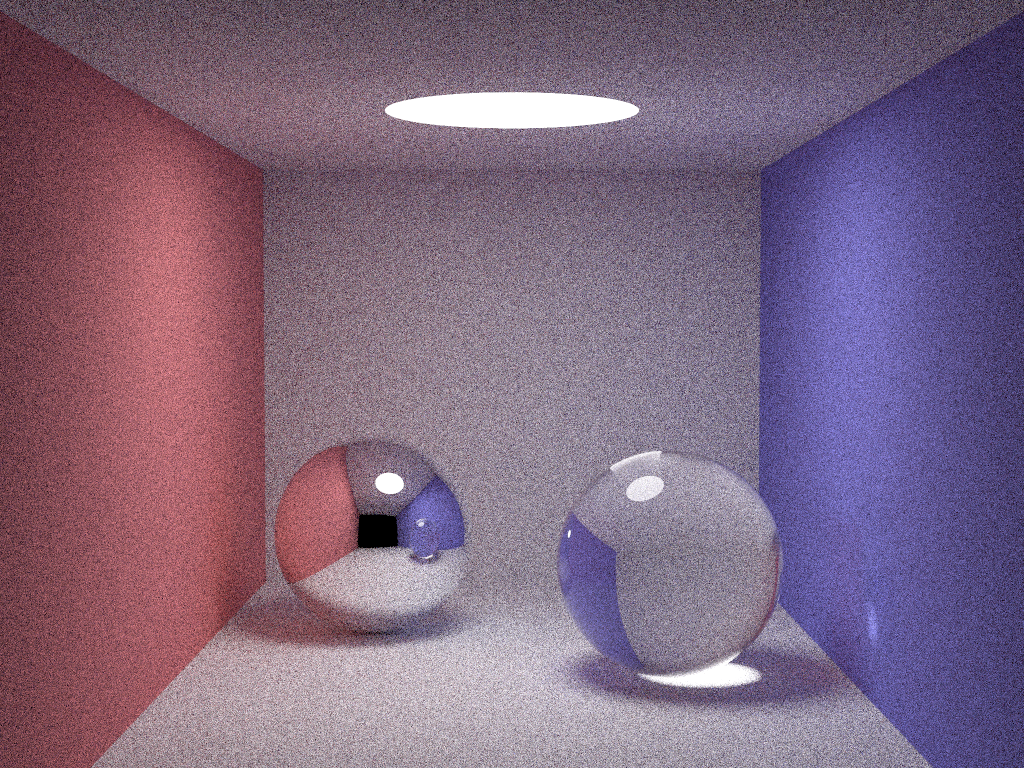
\includegraphics[width=\linewidth]{../assets/appendixD_result_200.png}
	\caption{200 campioni per stratum}
    \end{subfigure}\hfill
    \begin{subfigure}[c]{0.4\linewidth}
	\centering
	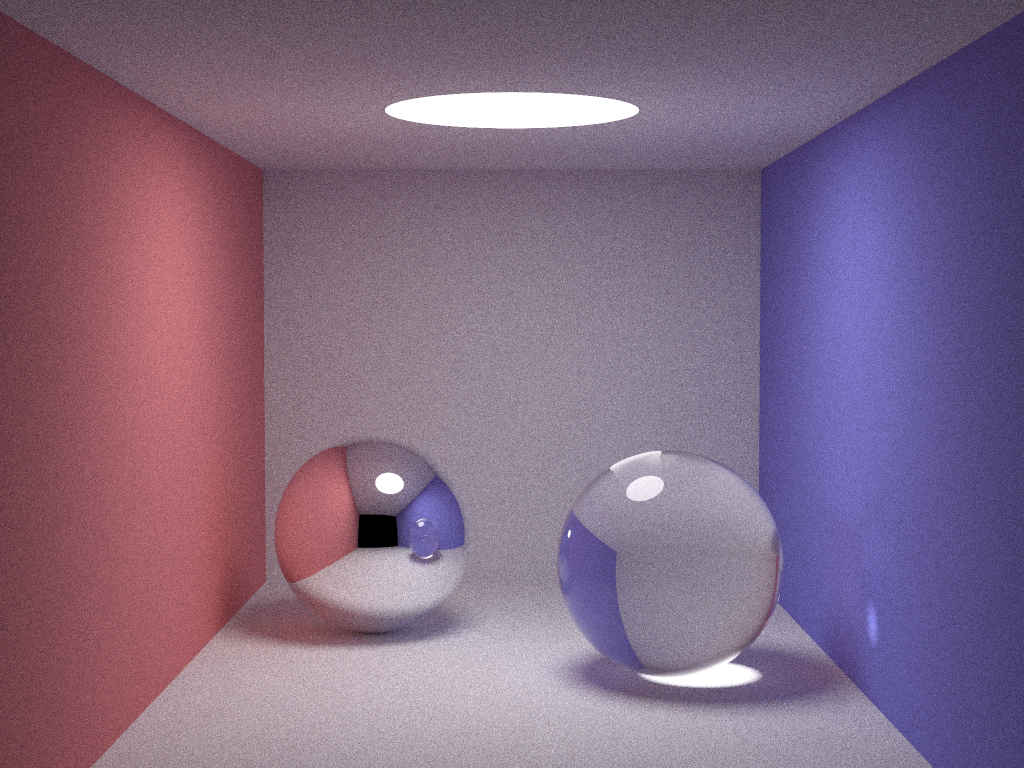
\includegraphics[width=\linewidth]{../assets/appendixD_result_1000.png}
	\caption{1000 campioni per stratum}
    \end{subfigure}\hfill
    \begin{subfigure}[c]{0.4\linewidth}
	\centering
	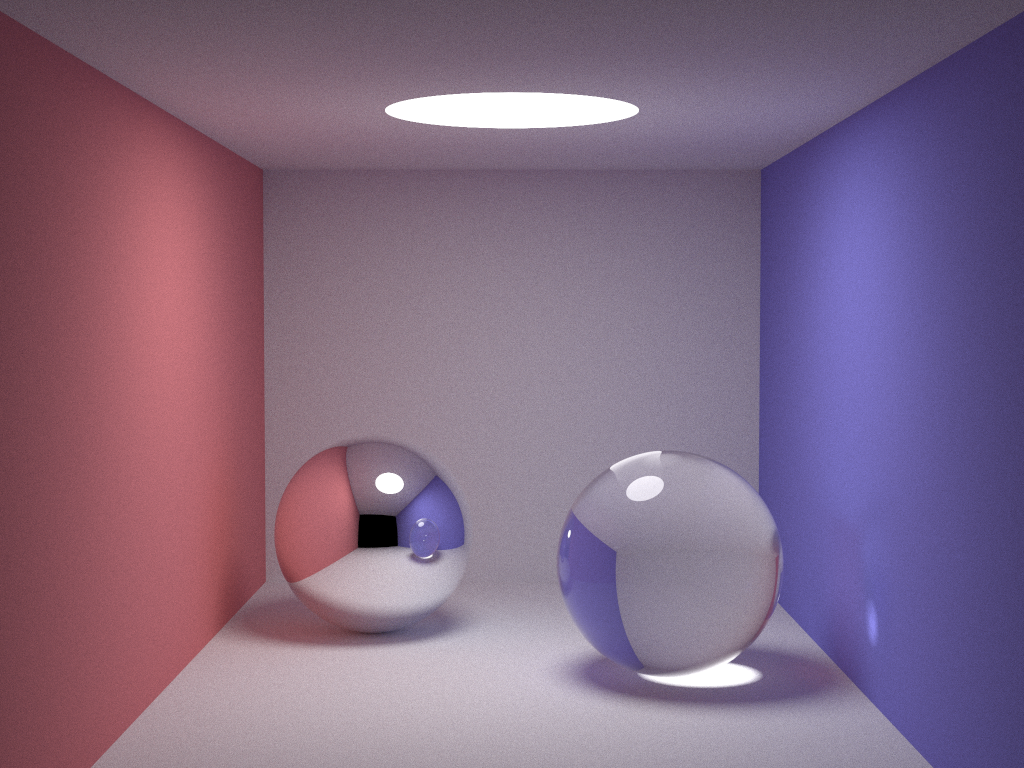
\includegraphics[width=\linewidth]{../assets/appendixD_result_5k.png}
	\caption{5000 campioni per stratum}
    \end{subfigure}\hfill
    \begin{subfigure}[c]{0.4\linewidth}
	\centering
	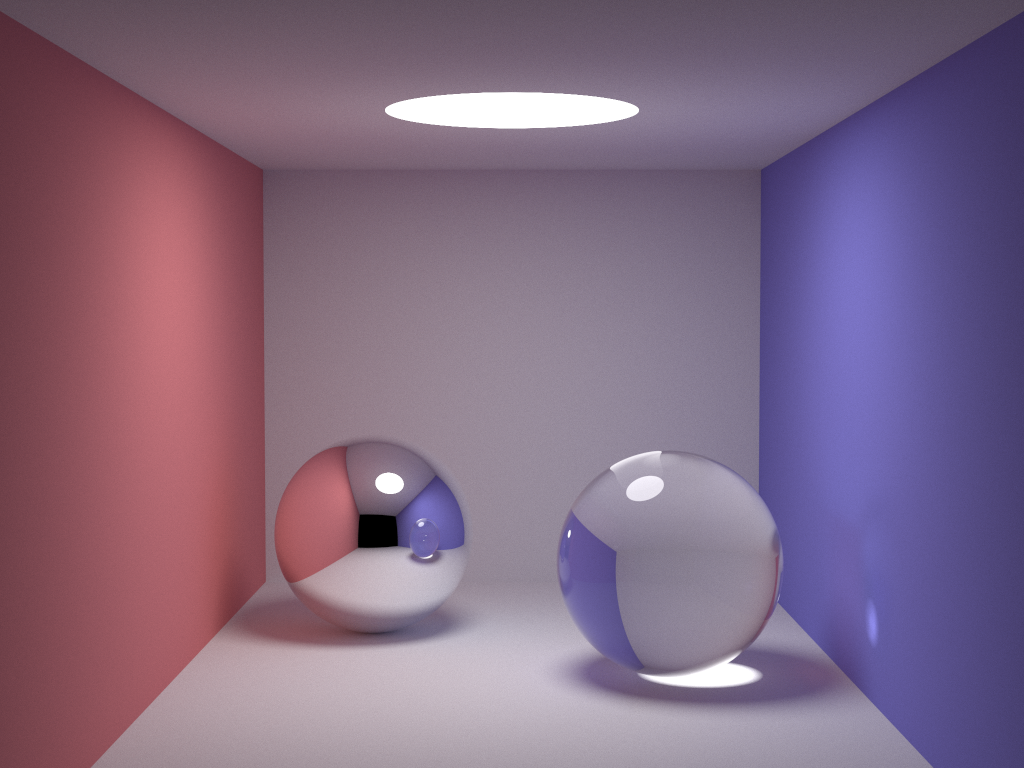
\includegraphics[width=\linewidth]{../assets/appendixD_result_25k.png}
	\caption{25000 campioni per stratum}
    \end{subfigure}
    \caption{Risultati dell'esecuzione dell'algoritmo con numero crescente di campioni per pixel}
	\label{chapter8:LT:results}
\end{figure}
Il codice completo pu\`o essere trovato in Appendice \ref{appendixD:pathTracer} assieme ai comandi per la compilazione.
\begin{table}[p]
	\begin{threeparttable}[b]
	\begin{tabularx}{\linewidth}{Yc}
		\toprule
		\multicolumn{2}{>{\hsize=\dimexpr2\hsize- + 2\tabcolsep\relax}X}
		{Varianza trovata per le immagini risultanti\tnote{1}} \\
		\midrule
		\multicolumn{2}{>{\hsize=\dimexpr2\hsize- + 2\tabcolsep\relax}X}{8 campioni per stratum}\\
		Red channel variance & 0.07344142 \\
		Green channel variance & 0.06190188 \\
		Blue channel variance & 0.07339846 \\
		Luminance variance & 0.06380390 \\
		\midrule
		\multicolumn{2}{>{\hsize=\dimexpr2\hsize- + 2\tabcolsep\relax}X}{40 campioni per stratum}\\
		Red channel variance & 0.05132978 \\
		Green channel variance & 0.04714374 \\
		Blue channel variance & 0.05175589 \\
		Luminance variance & 0.04621717 \\
		\midrule
		\multicolumn{2}{>{\hsize=\dimexpr2\hsize- + 2\tabcolsep\relax}X}{200 campioni per stratum}\\
		Red channel variance & 0.02482136 \\
		Green channel variance & 0.02453323 \\
		Blue channel variance & 0.02517796 \\
		Luminance variance & 0.02276842 \\
		\midrule
		\multicolumn{2}{>{\hsize=\dimexpr2\hsize- + 2\tabcolsep\relax}X}{1000 campioni per stratum}\\
		Red channel variance & 0.02023584 \\
		Green channel variance & 0.02019825 \\
		Blue channel variance & 0.02031221 \\
		Luminance variance & 0.01840096 \\
		\midrule
		\multicolumn{2}{>{\hsize=\dimexpr2\hsize- + 2\tabcolsep\relax}X}{5000 campioni per stratum}\\
		Red channel variance & 0.01904086 \\
		Green channel variance & 0.01936775 \\
		Blue channel variance & 0.01930308 \\
		Luminance variance & 0.01754279 \\
		\midrule
		\multicolumn{2}{>{\hsize=\dimexpr2\hsize- + 2\tabcolsep\relax}X}{25000 campioni per strata}\\
		Red channel variance & 0.01885027 \\
		Green channel variance & 0.01919554 \\
		Blue channel variance & 0.01911878 \\
		Luminance variance & 0.01737635 \\
		\bottomrule
	\end{tabularx}
	\caption{Tabella delle varianze}
	\label{chapter8:LT:variances}
	\begin{tablenotes}
		\item[1] {Ciascuna componente RGB \`e assunta normalizzata}
	\end{tablenotes}
	\end{threeparttable}
\end{table}
